\section{Architecture \& Methodology}
\label{chap:proposal:architecture}

As delineated in Section \ref{chap:introduction:objectives}, one of the dissertation's most important objectives is the secure exposure of network capabilities, allowing access to the funcionalities provided by the network in a controlled manner. The core network function responsible for the network capability exposure of a \acs{5G} system is the \acs{NEF}, as highlighted in Section \ref{sec:sba:nef}. Consequently, defining this component establishes the foundation for specifying the remainder of the network architecture. Due to the wide variety of \acs{5GC} implementations, an analysis of the various \acs{NEF} implementations was conducted in Section \ref{exposure:NEFimplementations}. Based on this analysis, the NEFSim~\cite{NEFSimMediaNetLabGithub} was selected as the most suitable choice for the \acs{NEF} implementation, due to its suite of supported northbound \acsp{API} and its integration capabilities with \acs{CAPIF} implementations (i.e. OpenCAPIF), compared to its alternatives.

In order to further simplify the access to the complex set of network services offered by the NEFSim, CAMARA \acsp{API} are adopted, providing an abstraction layer that facilitates the integration of network capabilities into applications. This way, the CAMARA initative supports the development of network applications that explore the wide variety of use cases enabled through its set of user-friendly \acsp{API}, as described in Section \ref{sec:iniatives:CAMARA}.

Hence, the CAMARA and NEFSim components handle the exposure of network capabilities to third parties. However, there is still a lack of a standardized mechanism for the secure discovery, exposure, and consumption of these northbound \acsp{API}, which is achieved through the introduction of \acs{CAPIF}. More specifically, OpenCAPIF~\cite{OpenCAPIF}, an open source project by the \acs{ETSI} \acs{SDG}, was selected for the implementation of the \acs{CAPIF} framework, due to its compliance with \acs{3GPP} standards and active support. Thus, OpenCAPIF will be utilized to securely expose CAMARA \acsp{API}, as well as \acs{NEF} \acsp{API}, to allow access to all NEF functionalities not supported by the CAMARA use cases or that have previously been used for implementation within \acs{ITAv}. Figure \ref{fig:system:architecture} illustrates the envisioned system architecture. It is adapted from a reference architecture by the SoftNet \acs{WG}, within the context of Smart Networks and Services Joint Undertaking, which establishes how a \acs{NaaS} platform enables third-party access to operator networks~\cite{SoftnetWhitePaperBaseArchitecture}. The baseline architecture was altered to the context of this dissertation, as well as to cater to functional specificities of the \acs{ITAv} testbed.


\begin{figure}[htbp]
    \centering
    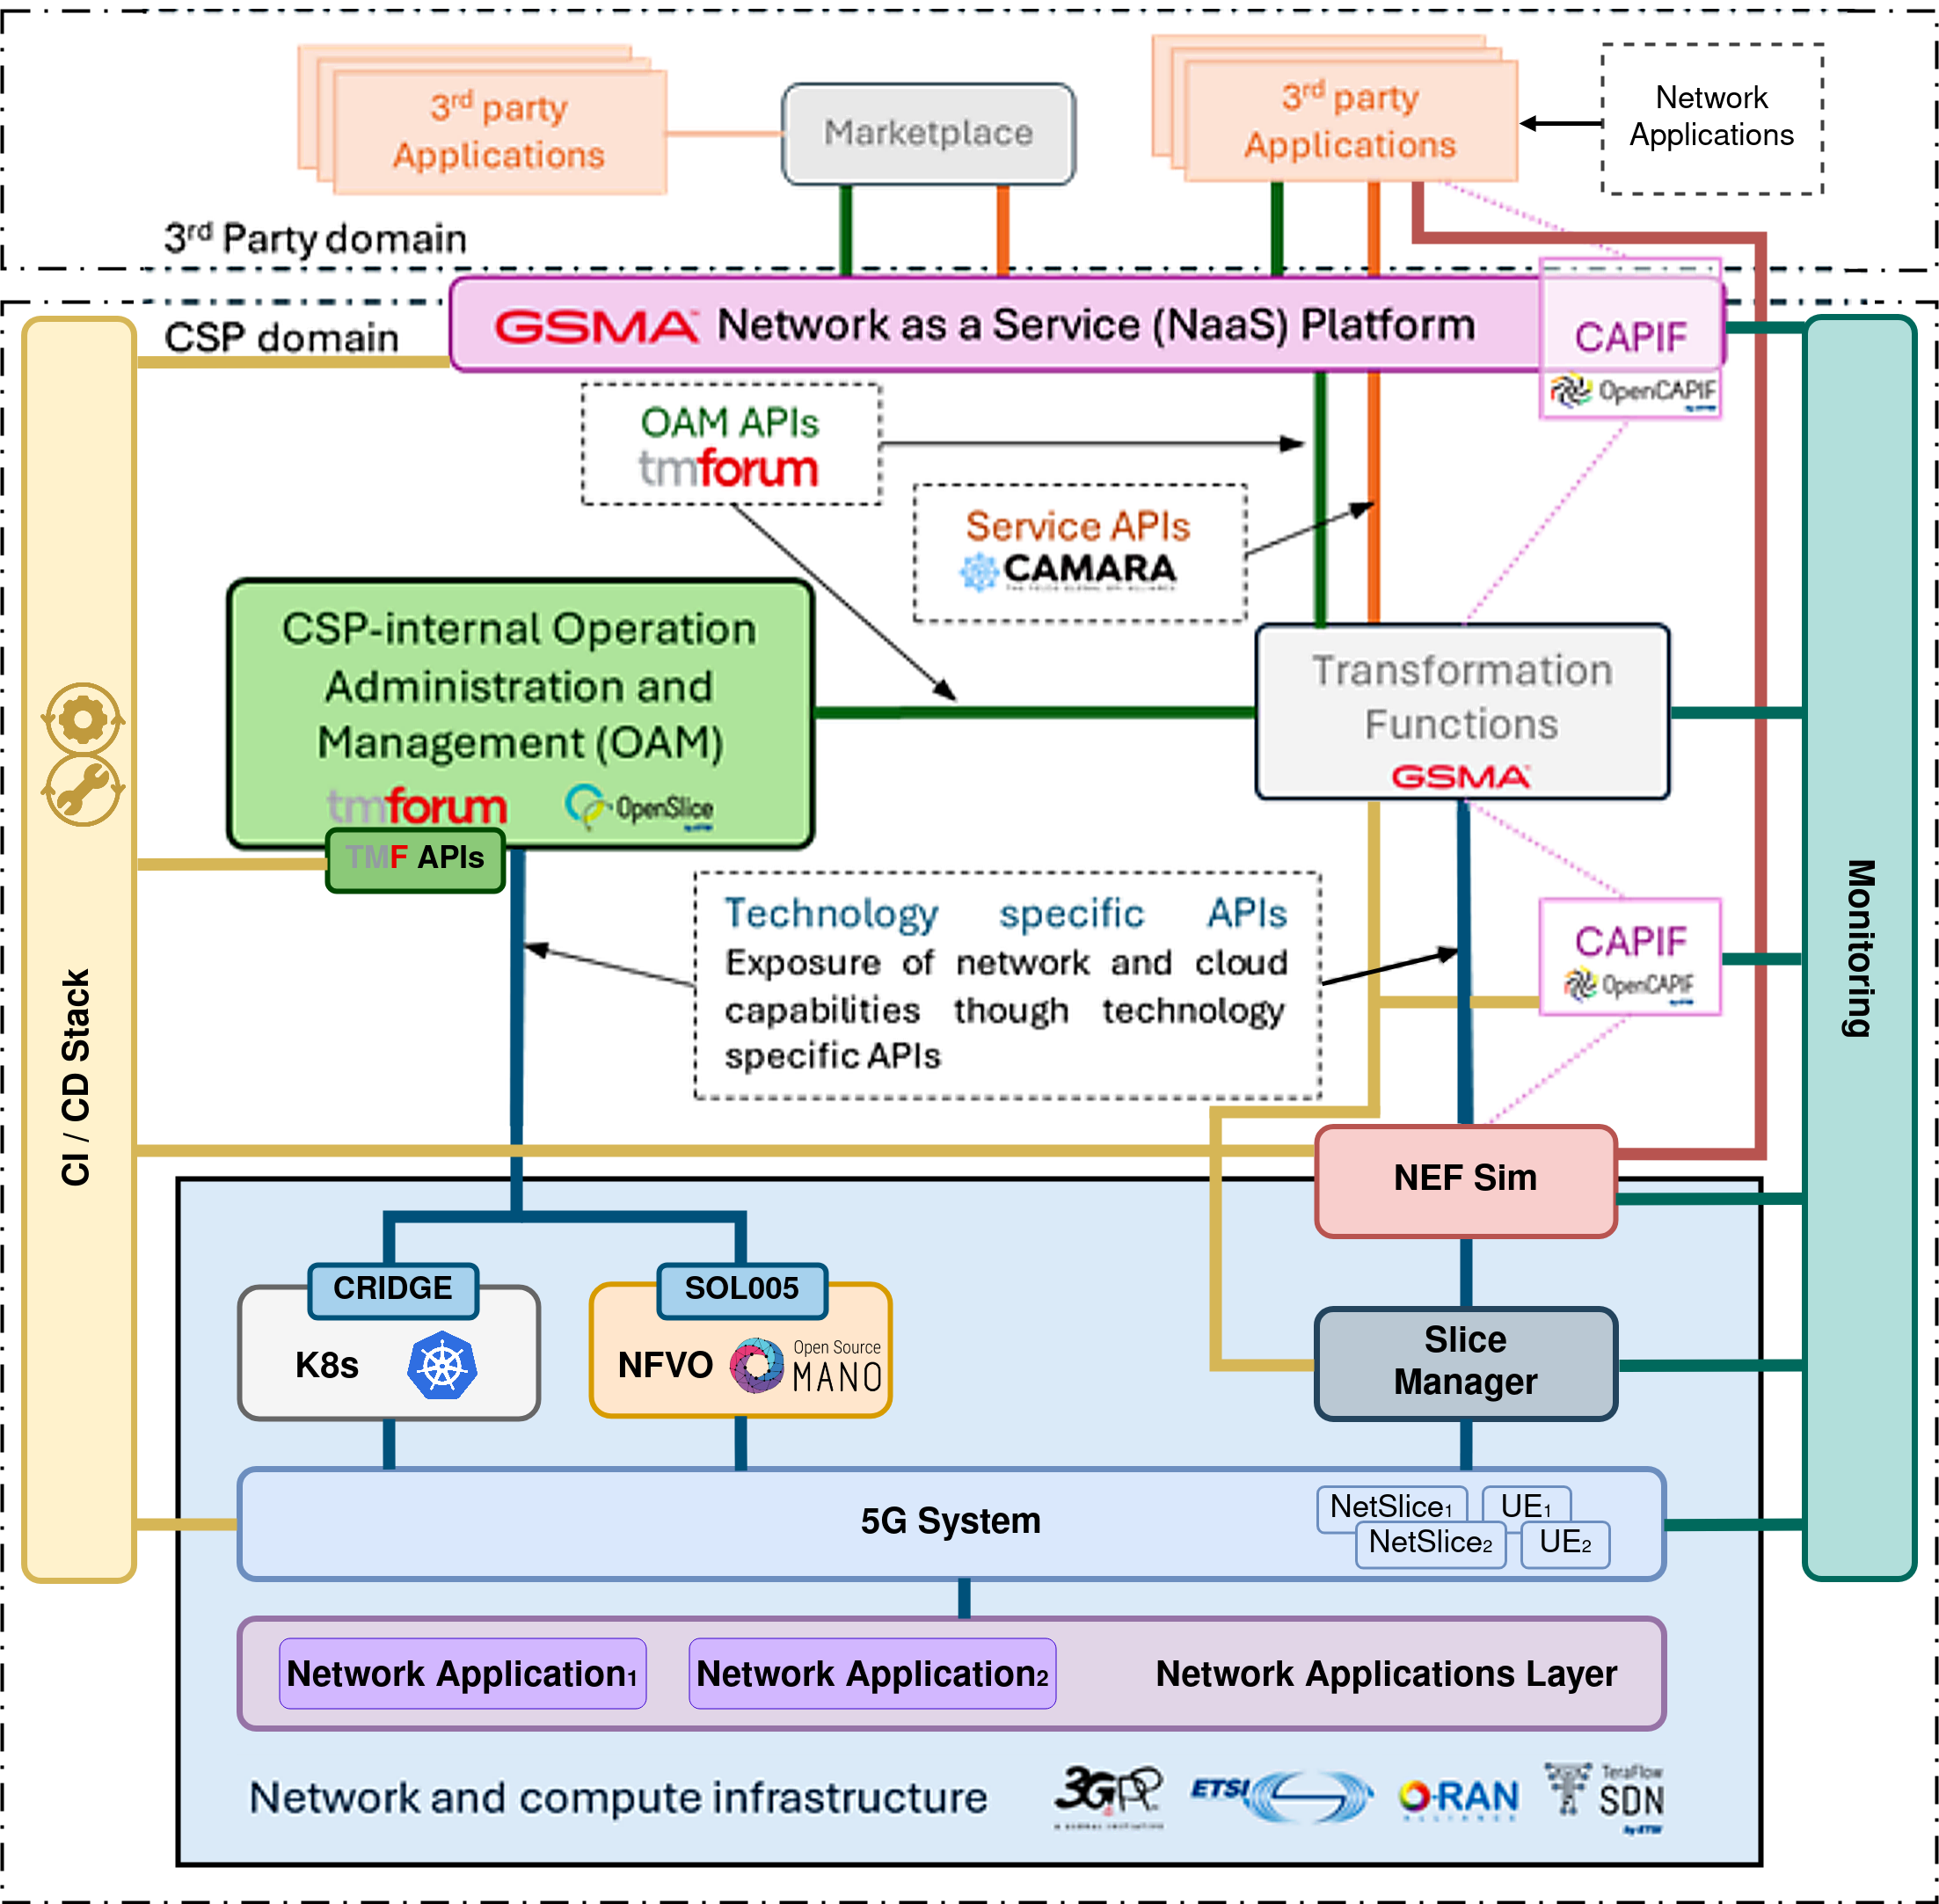
\includegraphics[width=1\linewidth]{figs/ThesisDiagram.png}
    \caption{Testbed Architecture}
    \label{fig:system:architecture}
\end{figure}

The combination of OpenCAPIF, \acs{NEF} and CAMARA provides standardized secure access to network capabilities across a wide range of use cases. To support this variety of use cases, network slicing should be applied to tailor to its heterogeneous service requirements on a common underlying infrastructure. To this end, \acf{OSL}~\cite{OpenSlice} is chosen as the predilect \acs{OSS} to deliver \acs{NaaS}, based on \acs{TMF} \acs{ODA}, since it's widely used in the literature for the provisioning and orchestration of \acs{5G} resources (especially \acsp{UE} and network slices) packaged as \acs{OSL} services, important for testing and validation purposes as showcased in Section \ref{sec:pipelines}. Nevertheless, \acs{OSL} is not an orchestrator, delegating the orchestration and provisioning of resources and network applications to the \acs{NFVO} \acs{OSM}, for \acs{NFV}-based deployment through the SOL005 interface, or to kubernetes, for containerized deployment through the CRIDGE component. \acs{OSL}, inspired by the Operator Pattern, also supports Generic Controllers to automate the lifecycle management of custom resources~\cite{OpenSliceGenericServicesController}. These can be leveraged to implement the lifecycle logic for the \acs{NSI} as discussed in Section \ref{sec:slice:lifecycle}, as well as that of the \acsp{UE}. Such Generic Controllers will be responsible for the creation, update and deletion of the aforementioned resources in the 5GAIner testbed by interacting with the proprietary \acs{ITAv} Slice Manager, which in turn interacts with the \acs{5G} System (\acs{5GC} and \acs{RAN}).

The implemented exposure interfaces, provided by the CAMARA and \acs{NEF} northbound \acsp{API}, and secured by OpenCAPIF, will serve as the foundation for the development and validation of future network applications, by a variety of developers. This should be achieved through an existing Continuous Integration and Continuous Testing platform, leveraging the \acs{TMF} Open \acsp{API} provided by \acs{OSL} to support the automated provisioning and lifecycle management of the required test components, such as \acsp{UE}, network slices and CAMARA \acsp{API}, followed by the execution of the test cases and collection of corresponding results.

It is also important to note  the existance of a telemetry monitoring stack utilizing Prometheus exporters and Grafana for the collection and visualization of the collected data, respectively, including metrics, logs and traces. Such telemetry stack can be encapsulated as a \acs{OSL} Service and provisioned for a specific test case. In paralell, a similar stack will be utilized to obtain monitoring information at a system level on static components that are not dynamically instantiated for individual test cases and are part of the 5GAIner testbed, namely, the NEFSim, Slice Manager and \acs{5G} system.

Lastly, a \acs{5G} Network Application will be developed leveraging the implemented exposure interfaces. This \acs{PoC} will cater to the specific requirements of the automotive vertical sector, interacting with OpenCAPIF, CAMARA and \acs{NEF} \acsp{API} to provide dynamic network-aware services. The Network Application will also be bundled as an \acs{OSL} service and integrated into a testing pipeline to verify the validity of the implemented functionality and system behavior.


